\documentclass{article}



\title{Multilevel Modeling of Infant Mortality in India*}
\author{Julian Bautista$\dag$\\
 \and
 Alexander Pavlakis$\dag$\\
 \and
 Advait Rajagopal$\dag$
 }
 \providecommand{\keywords}[1]{\textbf{Keywords --} #1}
\date{December 9 2016}
\setlength{\parindent}{0pt}

\usepackage{amsmath}
\usepackage{latexsym}
\usepackage{graphicx}
\usepackage{amsfonts}
\usepackage{wasysym}
\usepackage{amssymb}
\usepackage{mathrsfs}
\usepackage{multirow,array}
\usepackage{booktabs}
\usepackage{float}
\usepackage{color}
%
\usepackage[margin=1.25in,bottom=1in,top=1in]{geometry}
\usepackage{fancyhdr}
\pagestyle{fancy}
\usepackage{blindtext}

\lhead{}
\chead{Bautista, Pavlakis, Rajagopal}
\rhead{}
%\lfoot{\textit{STATGR6103 Final Project}}
\cfoot{}
\rfoot{\thepage}
\renewcommand{\headrulewidth}{1pt}
\renewcommand{\footrulewidth}{1pt}
%
\DeclareMathAlphabet{\mathpzc}{OT1}{pzc}{m}{it}
\linespread{1.4}
\usepackage{listings}
\usepackage[most]{tcolorbox}
\usepackage{inconsolata}
\newtcblisting[auto counter]{sexylisting}[2][]{sharp corners, 
    fonttitle=\bfseries, colframe=black, listing only, 
    listing options={basicstyle=\ttfamily,language=java}, 
    title=Listing \thetcbcounter: #2, #1}
    \newcommand\blfootnote[1]{%
  \begingroup
  \renewcommand\thefootnote{}\footnote{#1}%
  \addtocounter{footnote}{-1}%
  \endgroup
}
%%%%%%%%%%%%
%   Document starts   %
%%%%%%%%%%%%

\begin{document}
\maketitle
\blfootnote{$\dag${Department of Economics, The New School for Social Research}}
\blfootnote{*\textit{This is a working paper, please do not circulate or cite without permission.}}




\begin{abstract}
This paper studies infant mortality rates in Indian states from 2005 to 2014.  We identify state effects, time effects, and the impact of per-capita public health expenditure across states through Bayesian multilevel/hierarchical modeling. We validate our approach with posterior predictive checks. Once we account for state and time level variation explicitly, we find that percentage change in IMR with respect to percentage changes in per-capita health expenditure are small and negative (i.e they bring IMR down). State level effects however vary vastly and capturing this variation properly with partial pooling and weakly informative priors is a major breakthrough. We also consider the differential impact of per-capita health expenditure on female and male infants and find the patterns are different with more females dying across most time periods and most states.
\end{abstract}

\keywords{Bayesian multilevel modeling, hierarchical modeling, India, Infant Mortality, health expenditure, panel data}

\newpage

\tableofcontents
\newpage

%%%%%%%%%%%%
%      Introduction       %
%%%%%%%%%%%%

\section{Introduction}
\label{S:1}
The goal of this paper is to carry out a Bayesian multilevel analysis of Infant Mortality Rates (IMRs) and per-capita health expenditure in India. This model builds on an earlier approach \textcolor{gray}{[Rajagopal, 2016]} which which estimated the impact of health expenditure on IMR with a hierarchical model that controlled for state and time level variation. We choose 30 Indian states and Union Territories (UTs) in the period 2005 - 2014. We also consider the differential impact that health expenditure may have on the IMR of male and female infants.\\
Hierarchical modeling has two closely related meanings \textcolor{gray}{[Feller and Gelman 2015]}. First, hierarchies can explain a hierarchical data structure.  In this paper, IMR and health expenditure vary across states and over time, leading to a `panel' nature of the data. Second, hierarchies can also be used to describe how parameters are modeled, where the parameters of interests have their own distribution which are determined by a second level of parameters called hyperparameters. This kind of hierarchical modeling of parameters can be extended to more levels.\\
The multilevel modeling approach followed in this paper is its biggest contribution to the existing literature and particularly the body of study that has analyzed IMR and health expenditure in India. Past work has tended to rely on classical non-hierarchical approaches and methods that yield point estimates. Our hierarchical model properly takes into account state and time level variation in India. This is a major improvement because while previous studies have studied panel data, they often conclude with national level estimates. We believe that in order to really analyze state and time level variation in IMR and advocate policy in a more useful manner, a Bayesian multilevel analysis is a prerequisite.\\
The paper is organized as follows. In section two, we discuss some of the previous literature on the relationship between IMR and health expenditure. In section three, we briefly explain the intuition behind Bayesian hierarchical modeling, partial pooling and why they are steps forward in the analysis of data which varies spatially and across time. Section four explains the dataset, our sources, problems faced while building the dataset and necessary manipulations. We explain our dependent and independent variables and the reason for choosing them. It also has some guidelines that will help with reproducibility of our work. In section five we explore the dataset thoroughly. Here we try to highlight as many trends as possible in the variables of interest to give the reader and researchers a clear idea of how IMR and per-capita health expenditure have varied in India across time and the chosen states and UT's. Section six focuses on modeling and we explain the model specification and discuss its performance. Section seven provides the results of the model fitting exercise and shows the marginal posterior distributions of the relevant parameters and hyper parameters. We also show the results of posterior predictive checking in this section. Section eight concludes.\\

%%%%%%%%%%%%%%
%      Previous literature      %
%%%%%%%%%%%%%%
\section{Previous literature and similar studies}
\subsection{An overview of the issue}
Infant mortality is an important indicator of the level of human development and infrastructure in a country. Infant Mortality Rate can be defined as the number of deaths among infants aged less than one year in a given year as compared to 1000 live births in that same year \textcolor{gray}{[Central Intelligence Agency, 2014]}. Rich and poor countries naturally have very different levels of IMR. For instance the highest IMR was recorded in the WHO African Region (about 60) and the lowest IMR was recorded in the WHO European region (about 11) \textcolor{gray}{[World Health Organization 2013]} . India has an IMR of about 43 in 2014 and ranks 50$^{th}$ among 224 countries in descending order of IMR \textcolor{gray}{[Central Intelligence Agency, 2014]}. The reasons for infant mortality in rich and poor countries are also quite different. Infant mortality in rich countries is caused by birth defects, sudden death during infancy and premature births \textcolor{gray}{[McClead, 2012]}. In poorer countries on the other hand, improper sanitation, inadequate birth attendance, malnutrition, disease and lack of female education are some of the prevalent reasons for higher rates of infant mortality. \textcolor{gray}{[Filmer and Pritchett, 1999; Bidani and Ravallion, 1995; Bhat and Jain, 2004; Bhalotra, 2007; Kumar, et al., 2013]}. This paper however considers public health expenditure as the important factor explaining the pattern of infant mortality. As Barenberg et al. \textcolor{gray}{[2016]} point out, India's historically low levels of public health expenditure and highly privatized healthcare system could be important factors limiting human development and quality healthcare. India is a large country with very diverse geographical and demographic features and this influences the rural and urban nature of the population. While there are often hospitals and healthcare providers available in the larger urban cities, as Schultz \textcolor{gray}{[1993]} points out, it is often low income, rural, agricultural households that have higher mortality rates. In several rural areas, the concept of the midwife, distrust of hospitals and poor maternal health lead to the deaths of infants at or soon after birth. These differential trends across geographical regions within India is a major reason why classical statistics fails to analyze the problem of infant mortality. Classical or frequentist estimates are based on either complete pooling (all states are homogenous units) or no pooling (all states are heterogenous units). The truth lies somewhere in between and thus the idea of partial pooling with a Bayesian hierarchical model becomes a very important methodological advancement in studies like this one. 
\subsection{Contrasting studies}
Past studies, which have tried to answer the question ``does health expenditure impact infant mortality?" have often come up with conflicting results. Some researchers \textcolor{gray}{[Filmer and Pritchett, 1999; Musgrove, 1996]} say that public health spending does not have a significant impact (or has very little impact) on reducing infant mortality. Another group of researchers though, have found a significant impact of health expenditure on IMR \textcolor{gray}{[Farahani et. al, 2010; Bhalotra, 2007; Anand and Ravallion, 1993]}. Studies that have used panel data sets for the Indian states often report no significant relation between the two variables (IMR and health expenditure). A good summary of these studies is also available in Barenberg et al. \textcolor{gray}{[2016]}. However it is very important to note that often the differential points of view arise from different samples being considered. Many authors argue that  restricting samples to developing countries and poorer households might tell a very different story.  Authors who have researched the relation between Infant Mortality or probability of mortality and health expenditure have arrived at a similar conclusion when they carried out cross national studies limited to poorer countries, that the poorer countries and poverty stricken households have much more to gain from state or national level health expenditure \textcolor{gray}{[Farahani et al. 2010; Bhalotra, 2007; Schultz, 1993]}. Some research also shows that incremental health spending on prenatal care, proper child birth attendance, immunization and effective management of malnutrition and disease will bring down IMR \textcolor{gray}{[Kumar et al. 2013;  Bhalotra, 2007; Bidani and Ravallion, 1995]}.  In this context, more individual level variables like ``per-capita health expenditure" are much more important than macro level variables like ``percentage of state GDP allocated to healthcare" as Barenberg et al. \textcolor{gray}{[2016]} have used. Moreover they use a panel data analysis with information across time and states to come up with a pooled national level estimate, but this is insufficient as different states have their own unique problems. Policy-makers need to account for this and tackle healthcare issues differently based on where they are and what the existing barriers to human development might be there.  National level or aggregate studies fall short in this area.\\


\subsection{The gender component}
Upon closer examination of the data we found that the number of female infant deaths almost always outnumbers the number of male infant deaths. This is a pattern consistent across states both rich and poor and across all time periods. Some of these trends have been represented graphically in Figure 3 and Figure 4 in Section 5. This led us to believe that considering merely infant mortality which appears to be computed as an average of male and female infant deaths was insufficient and we carry out a parallel study where the dependent variable is male and female infant mortality and compare the results of the two studies across the 30 chosen geographical regions and time period from 2005 - 2014. \\
There are several studies that highlight some of the problems for women and particularly female children and infants. India has been known to have a chronic sex preference that is so strong that it often endangers the lives of young women and children \textcolor{gray}{[Miller, 1981]}. It is also observed that there is a greater degree of freedom for women in south India when compared to the North. This again dials back to the question of geographic heterogeneity. There are striking regional imbalances in the status of women in society \textcolor{gray}{[Bardhan, 1982]}. While women have higher levels of education and literacy, this allows them better access to healthcare and allopathic medicine which directly culminates in better pre and post natal care. Education of women is an important driving force behind reduced infant and child mortality. In India women are seen to have a higher mortality at almost every age and in particular childhood \textcolor{gray}{[Bourne and Walker, 1991]}. We have seen (and shown graphically) that this trend of higher female mortality persists among infants. This is a worrying trend and has been a concern for Indian policy-makers. However econometric research in infant mortality has often failed to address this aspect of the problem and we believe this needs to be investigated more thoroughly.\\

The primary advancements made by this paper are in the realm of statistical methodology and a study of gender disparities in infant mortality. Our usage of partial pooling and Bayesian multilevel modeling is ideal for this kind of a problem and our separation of the problem into female and male infant deaths are the gaps in research which we hope to bridge.




%%%%%%%%%%%%%%%%
%     Hierarchical modeling      %
%%%%%%%%%%%%%%%%
\section{Bayesian multilevel (hierarchical) modeling and partial pooling}
The steps of a full Bayesian data analysis as described by  Gelman et. al \textcolor{gray}{[2013]} and followed in this paper are as follows;
\begin{enumerate}
\item{Set up a full probability model that is a joint probability distribution encompassing all observed and unobserved quantities. This model should reflect prior knowledge of the problem at hand and should account for the method of data collection}
\item{Estimate the posterior distribution conditional on prior knowledge and the observed data.}
\item{Check the fit of the model and the resulting implications of the posterior parameter estimates.}
\end{enumerate}
There is an underlying assumption that the explanatory variable only affects the distribution of the dependent variable through the explanatory variable itself. This implies that the conditional distribution of the dependent variable is independent of the marginal distribution of the explanatory variable.\\
The primary advantage of partial pooling in this paper is to improve on the classical estimates used in previous literature and similar panel studies. The classical estimates are either complete pooling or no pooling analyses. Complete pooling provides a single estimate for the whole country from the panel dataset and a no pooling approach regards each state as an independent unit. This is where a multilevel Bayesian model with partial pooling performs very well.  Multilevel modeling as such, is a generalization of regression methods and is usually an improvement over classical regression methods. It can improve prediction and be helpful for causal inference  \textcolor{gray}{[Gelman, 2006]}.
We also impose Bayesian priors on our parameter estimates. This has the dual advantage of allowing inherent subjectivity to be captured in the model and preserves the hierarchical structure. Priors are information that we get from previous or similar studies, subject matter experts or results from related disciplines. Priors also restrict the parameter space the Hamiltonian Monte Carlo algorithm has to traverse in order to converge on the target distribution. We want to use appropriately informative priors,  so as to not overshadow the data with very strong prior information \textcolor{gray}{[Gelman et al. 2013]}.  In our case each state and time period has its own effect but these parameters are realizations from a state level and time level prior distribution (for more information about the hierarchical structure of the model, see Section 6).


%%%%%%%%%%%%%%
%      Explaining Data       %
%%%%%%%%%%%%%%


\section{The dataset and relevant variables}
Our goal is to estimate the functional relationship between IMR and state-wise per-capita health expenditure.  The time period we have taken into consideration is 2005 - 2014. This is a short time period but it must be noted that reliable numbers are only available for this period for the thirty states and UT's under consideration. The regions we do not consider due to partial or complete unavailability of data are ``Andaman and Nicobar Islands", ``Daman and Diu", ``Dadra and Nagar Haveli", ``Lakshadweep", ``Chandigarh" and ``Telangana".\\
The Sample Registration System's (SRS) Census Data  \textcolor{gray}{[Ministry of Home Affairs, Government of India, 2014]} provides a detailed account of all vital statistics collected in the country. The IMR data comes from the SRS bulletins. We retrieved state-wise average IMR as well as male and female IMR for the purpose of our study. This is the dependent variable.  Health expenditure is measured using `per-capita health expenditure' -- total health expenditure divided by the population.  The data on health expenditure comes from the Reserve Bank of India's State Budget publications. Per-capita health expenditure is our main predictor variable. The final dataset is a balanced panel dataset with 300 observations (30 states $\times$ 10 time periods).\\
 We use per-capita health expenditure lagged by one period because it is understandable that incremental expenditure in the previous period will impact IMR in the current period. This is an improvement over many other similar works in this field of study because they use expenditure in the current period. This transformation leaves 270 observations.\\
The total state and UT health expenditure is the ``Revenue Expenditure of States and Union Territories'' allocated to ``Medical and Public Health"  \textcolor{gray}{[Reserve Bank of India, State Finances]}. The population for states comes from the 2011 Indian Census. We use the annual population growth rate to approximately calculate the population in the thirty states and UT's in the given time period. Then we divide total health expenditure by population to obtain per-capita health expenditure.\\


%%%%%%%%%%%%%%%%%%%%%
%      Exploratory analysis and trends     %
%%%%%%%%%%%%%%%%%%%%%
\section{Exploratory data analysis and trends in the data}
\subsection{Comparing IMR in 2005 and 2014}
\begin{figure}[H]
   \begin{center}
   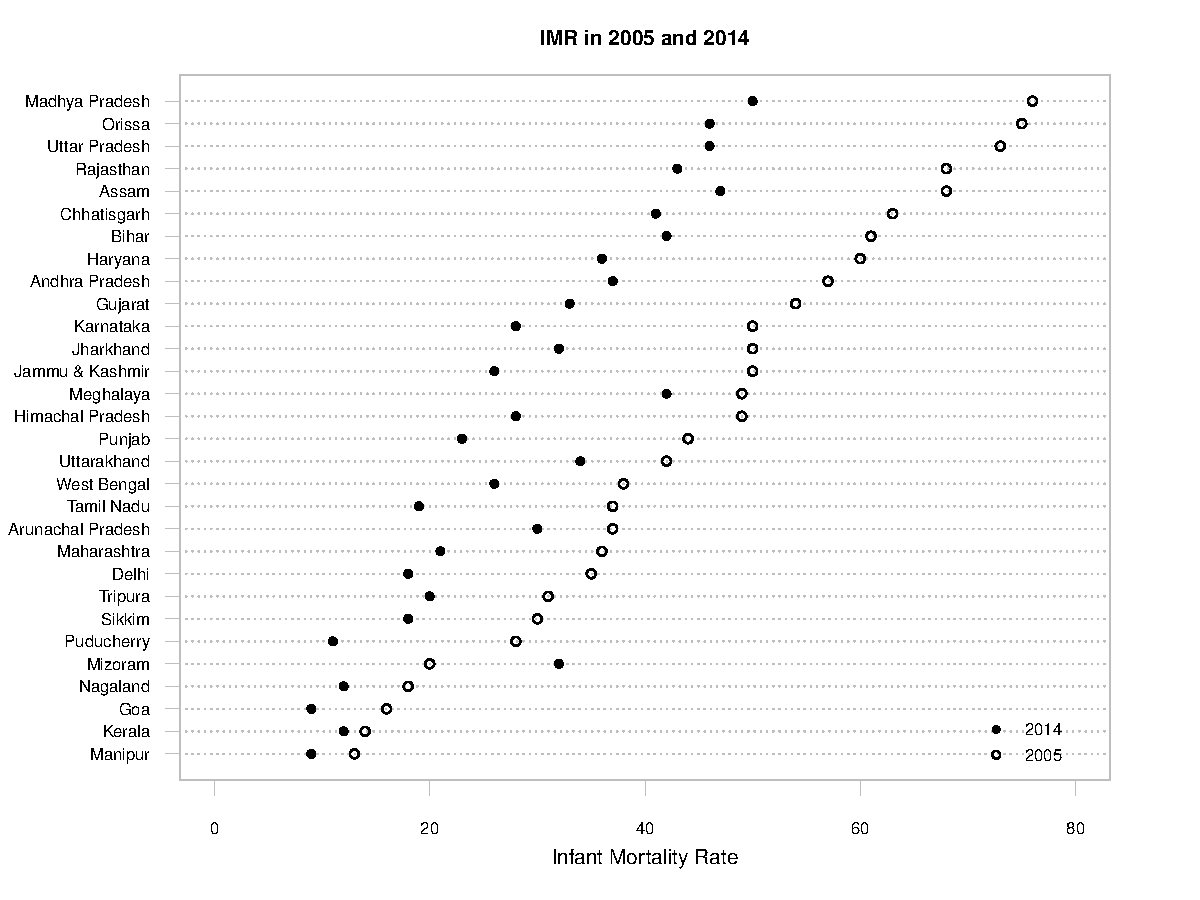
\includegraphics[scale = .8]{compare_05_14.pdf}
   \end{center}
   \caption{\emph{Infant Mortality Rates by state in 2005 and 2014. The dots are the IMR in 2014 and the circles are IMR in 2005.}}
\end{figure}
There is wide variation in IMR across states and over time. Figure 1 displays IMR by state in 2005 and 2014.  All states (with the exception of Mizoram) showed improvement in IMR between 2005 and 2014.  States that had higher IMR in 2005, such as Madhya Pradesh, tended to have large decreases in IMR by 2014.  States with lower IMR in 2005, such as Manipur, tended to have smaller  decreases in IMR by 2014.  The data are roughly consistent with a constant decline among states between 2005 and 2014.

\subsection{IMR in the 30 regions from 2005 to 2014}
\begin{figure}[H]
   \begin{center}
   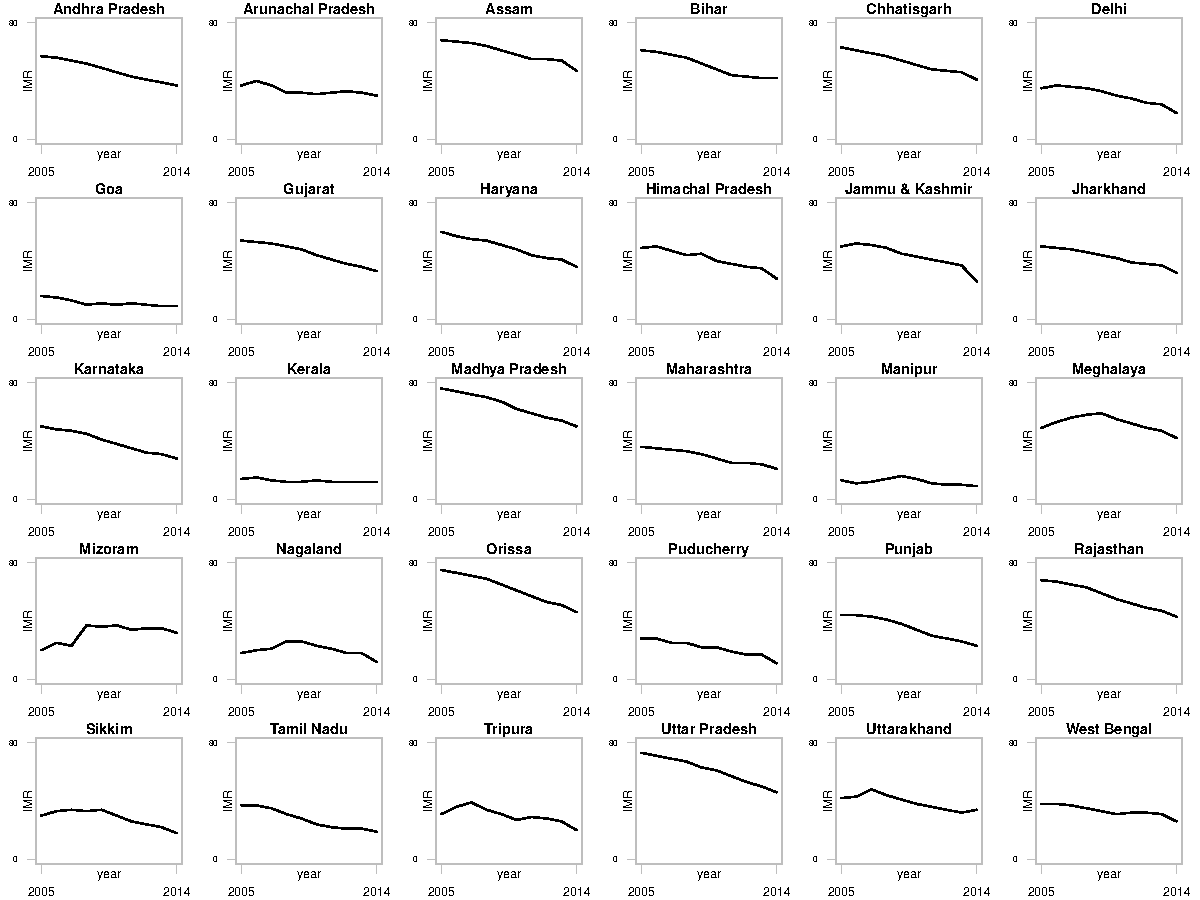
\includegraphics[height = 11cm, width = 15cm]{state_imr.pdf}
   \end{center}
   \caption{\emph{The horizontal axis represents years from 2005 to 2014. The vertical axis measures the IMR. The black lines show the trend in IMR.}}
\end{figure}
Figure 2 displays IMR over time for each state individually.  IMR appears to be generally decreasing in all states, but from different levels and at different rates.  In some states, such as Uttarakhand, IMR increases for a period before decreasing. Patterns in IMR that raise concerns are Assam, Bihar, Jharkhand, Orissa and Uttar Pradesh because while they have declined they are much higher than the absolute IMR levels in other states of similar size and population.

\subsection{IMR for females and males in the 30 regions from 2005 to 2014}
\begin{figure}[H]
   \begin{center}
   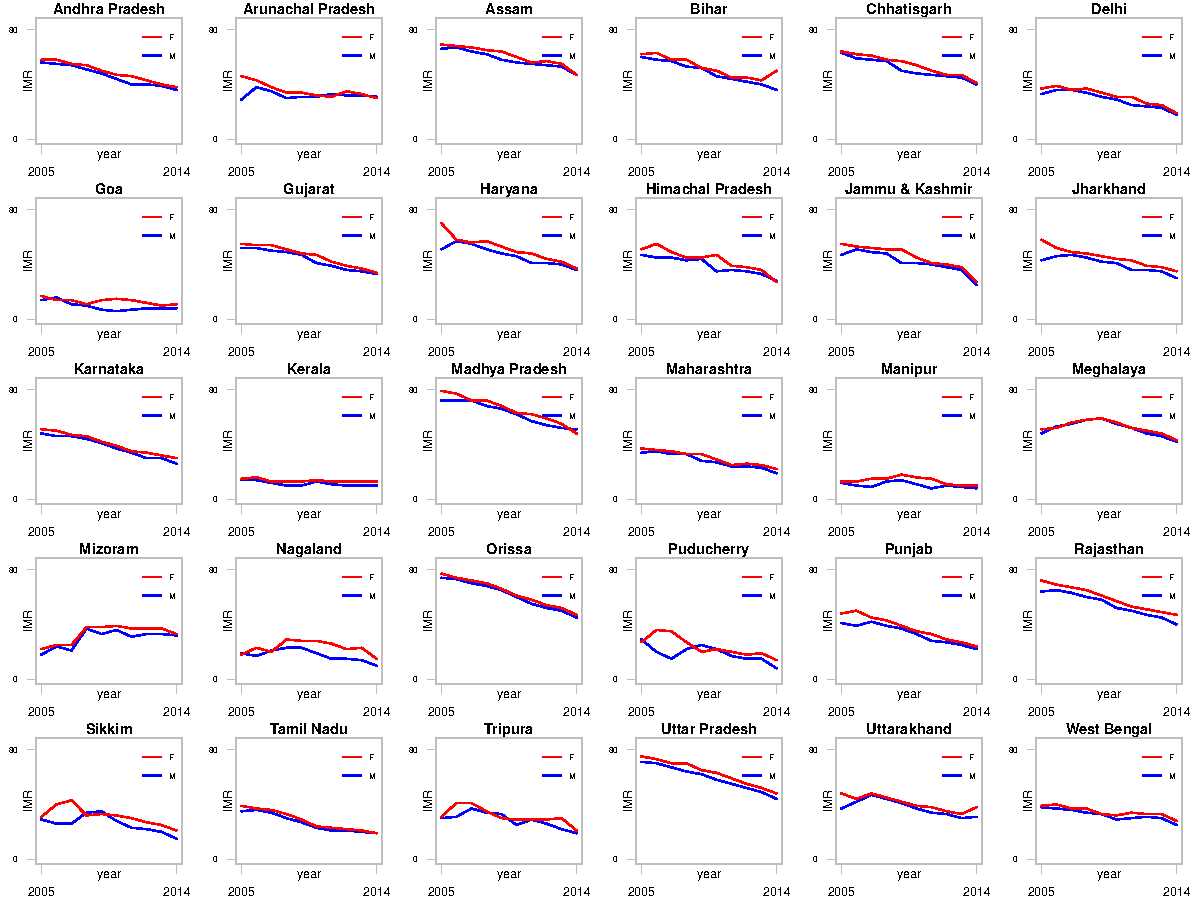
\includegraphics[height = 11cm, width = 15cm]{fem_mal.pdf}
   \end{center}
   \caption{\emph{The horizontal axis represents years from 2005 to 2014. The vertical axis measures the IMR. The red lines show the trend in female IMR and the blue lines show the trend in male IMR .}}
\end{figure}
 
Figure 3 displays IMR by gender and by state over time.  It shows how male and female IMR have similarities but follow distinct trends. It shows that female IMR is greater than male IMR in most states and in most years. This is worth highlighting as an interesting trend, mostly because even though IMR numbers decline, the red line for female IMR is almost always above the blue line for males.

\subsection{Ratio of female to male IMR in the 30 regions from 2005 to 2014}
\begin{figure}[H]
   \begin{center}
   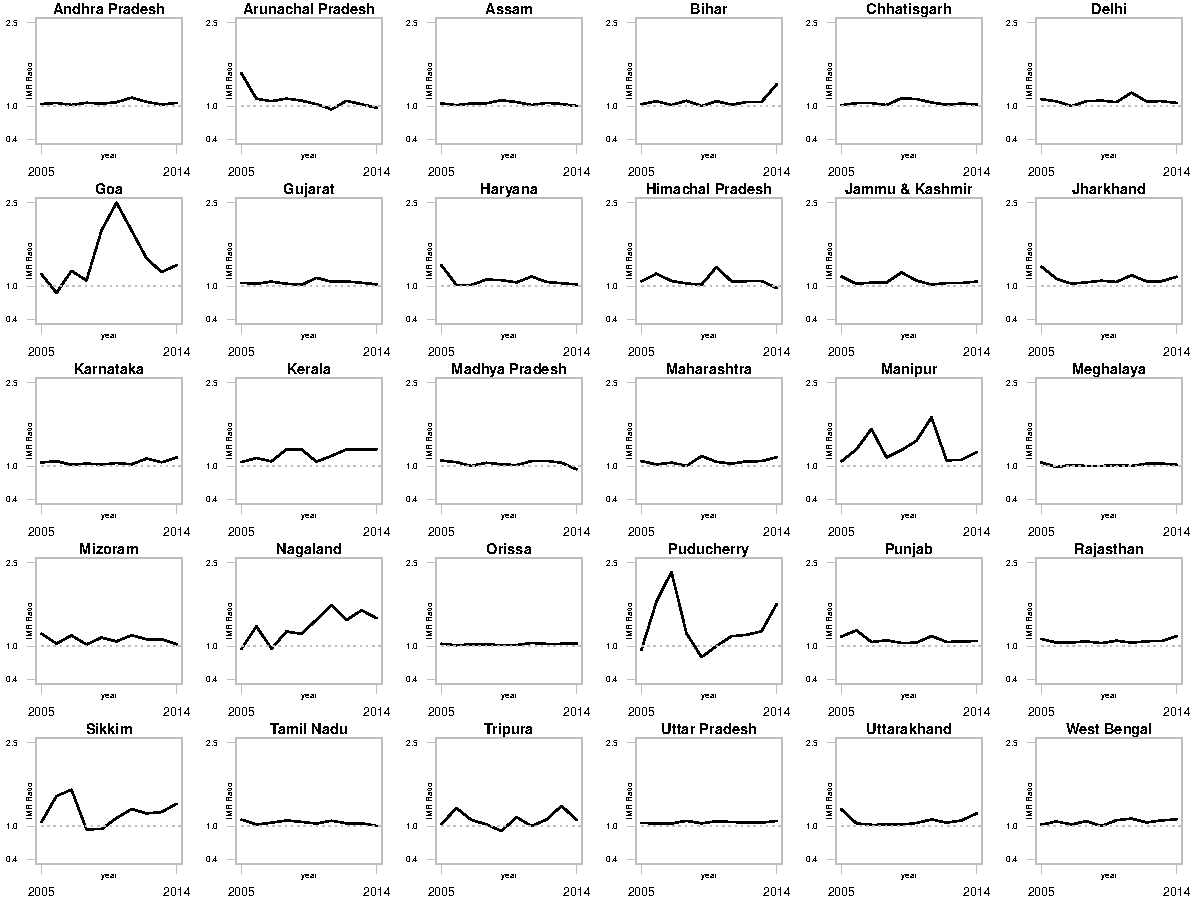
\includegraphics[height = 11cm, width = 15cm]{ratio.pdf}
   \end{center}
   \caption{\emph{The horizontal axis represents years from 2005 to 2014. The vertical axis measures the ratio of IMR. The dotted gray line is at 1. The black line shows the trend in the ratio of female to male IMR.}}
\end{figure}

Figure 4 shows the ratio of female to male IMR for the 30 regions in the time period 2005 - 2014. Wherever the black line is above the dotted gray line is where the number of female infants dying is greater than the number of male infants dying. We see sudden spikes in the black line in states like Goa, Puducherry, Sikkim and Manipur. These spikes are indicative of periods where the number of female infants dying far outnumbers the male infants dying. This is another way to view the information contained in Figure 3 which shows the consistent disparity in the number of female and male deaths.

\newpage

%%%%%%%%%%%%%%%%%%%%
%      Model specs and explanation     %
%%%%%%%%%%%%%%%%%%%%
\section{Model specification and explanation}
Our goals in modeling these data are to identify state-level effects on IMR, to identify year-level effects on IMR, to identify the impact of per-capita health expenditures on IMR, and to gauge if these effects are different between males and females. In order to capture the difference in trends for male and female infants we run the model for male and female infants and compare the results.\\ 

We assume a normal linear regression model for the likelihood function. $IMR_{st}$ is the dependent variable and represents the infant mortality rate in state `s' at time `t'. The predictor is $health_{st-1}$ and it represents per-capita ``revenue expenditure on medical and public health", in state `s' and time `t-1' (lagged by one period).  Since the dependent and predictor variable are confined to the positive real space we take a logarithmic transform, in classical terms this is a log - log regression. The advantage this provides is that the estimated parameter of interest ($\beta_s$) is an elasticity that will measure percentage change in IMR relative to percentage changes in health expenditure. The complete normal model is as follows: \\
 \begin{equation}
    \displaystyle
     \text{log}(IMR_{st}) \sim  \mathcal{N}(\alpha_s + \alpha_t + \beta_s \cdot \text{log}(health_{st-1}), \sigma^2)
    \end{equation}  
    \begin{align}
    \displaystyle
    \alpha_s \sim  \mathcal{N}(\mu_{\alpha_s}, \tau_{\alpha_s}^2) \\
    \alpha_t \sim  \mathcal{N}(\mu_{\alpha_t}, \tau_{\alpha_t}^2) \\
    \beta_s \sim  \mathcal{N}(\mu_{\beta_s}, \tau_{\beta_s}^2)    
  \end{align}
Equation 1 is the likelihood function. Equations 2, 3 and 4 are the prior distributions on the parameters $\alpha_s, \alpha_t$ and $\beta_s$. $\alpha_s$ is the state level intercept and $\alpha_t$ is the time level intercept. $\beta_s$ is the state level elasticity of IMR with respect to changes in health expenditure. This is a varying-coefficient model and exchangeability of the units of analysis is built into the model. We ensure exchangeability by conditioning on indicators that correspond to states and time periods and represent groupings in the population. This allows each subgroup to have a different mean outcome level  \textcolor{gray}{[Gelman et. al 2013]}. The exchangeability of time periods is therefore problematic but given the small period of time under consideration we do not expect any substantial structural differences . We observe that the posterior predictive checks work and since we have no reason to believe that any one year is vastly different than the others we go ahead with the assumption of exchangeability. We also impose normal priors on the hyperparameters $\mu_{\alpha_s}, \mu_{\alpha_t}$ and $\mu_{\beta_s}$ and half-Cauchy priors on all variance parameters (i.e $\sigma, \tau_{\alpha_s}, \tau_{\alpha_t}$ and $\tau_{\beta_s}$) because the half-Cauchy has a broad peak at zero and with a sufficiently large scale behaves as a weakly informative prior distribution  \textcolor{gray}{[Gelman 2006]}.


\newpage
%%%%%%%%%%%%%%%%%%%%%%
% Results and posterior predictive checks %
%%%%%%%%%%%%%%%%%%%%%%
\section{Results and posterior predictive checking}
Subsection 7.1 and 7.2 show the mean and quantiles of the marginal posterior distributions of the hyperparameters for males and females. Subsection 7.3, 7.4 and 7.5 are posterior predictive checking. Subsection 7.6 shows the state level intercepts for females and males. Subsection 7.7 shows the marginal posterior distribution of the elasticity parameter $\beta_s$ separately for females and males.
\subsection{Summary statistics of hyperprior distributions - Females}
\begin{table} [H]
\caption{Posterior Distributions of relevant parameters: Female}
\vspace{2mm}
\def\arraystretch{1}
\centering \begin{tabular}{c c c c c c c c} 
\hline\hline 
\vspace{1mm}
 & mean  & 2.5\%  &  25\% &   50\% &   75\% & 97.5\% &  \\  [0.5ex] \hline
$\mu_{\alpha_s}$ & 2.79 &  1.68 &  2.30 &  2.78 &  3.28  & 3.91   \\
$\tau_{\alpha_s}$  &  0.73  & 0.37  & 0.58 &  0.72 &  0.86 &  1.13    \\
$\mu_{\alpha_t}$ & 1.26  &  0.29  & 0.76 &  1.24  & 1.72  & 2.33      \\
$\tau_{\alpha_t}$ &  0.14  &  0.08  & 0.11 &  0.13  & 0.16  & 0.26   \\
$\mu_{\beta}$ &   -0.08   & -0.16  & -0.10 &  -0.08  & -0.05 &  0.01   \\
$\tau_{\beta}$ &  0.10  &  0.04 &  0.08 &   0.10 &  0.12  & 0.16  \\
$\sigma$ & 0.09 & 0.08 &  0.09 &  0.09  & 0.09 &  0.10 \\
\hline 
\end{tabular}
\end{table}

\subsection{Summary statistics of hyperprior distributions - Males}
\begin{table} [H]
\caption{Posterior Distributions of relevant parameters: Male}
\vspace{2mm}
\def\arraystretch{1}
\centering \begin{tabular}{c c c c c c c c} 
\hline\hline 
\vspace{1mm}
 & mean  & 2.5\%  &  25\% &   50\% &   75\% & 97.5\% &  \\  [0.5ex] \hline
$\mu_{\alpha_s}$ & 2.37 &  1.32 &  1.86  & 2.34 &  2.85 &  3.55  \\
$\tau_{\alpha_s}$  &  0.51  & 0.34 &  0.44  & 0.51  & 0.57 &  0.73    \\
$\mu_{\alpha_t}$ & 1.20  &  0.27 &   0.68  & 1.18  & 1.68 &  2.35        \\
$\tau_{\alpha_t}$ &  0.18  &  0.10  & 0.14  & 0.17  & 0.20  & 0.33  \\
$\mu_{\beta}$ &   -0.02   & -0.11 & -0.05 & -0.01 &  0.02  & 0.07   \\
$\tau_{\beta}$ &  0.05  &   0.01  & 0.04  & 0.05 &  0.06 &  0.09 \\
$\sigma$ & 0.11 & 0.10 &  0.11 &  0.11  & 0.12 &  0.13 \\
\hline 
\end{tabular}
\end{table}


\subsection{Posterior predictive checking of female and male IMR}
\begin{figure}[H]
   \begin{center}
   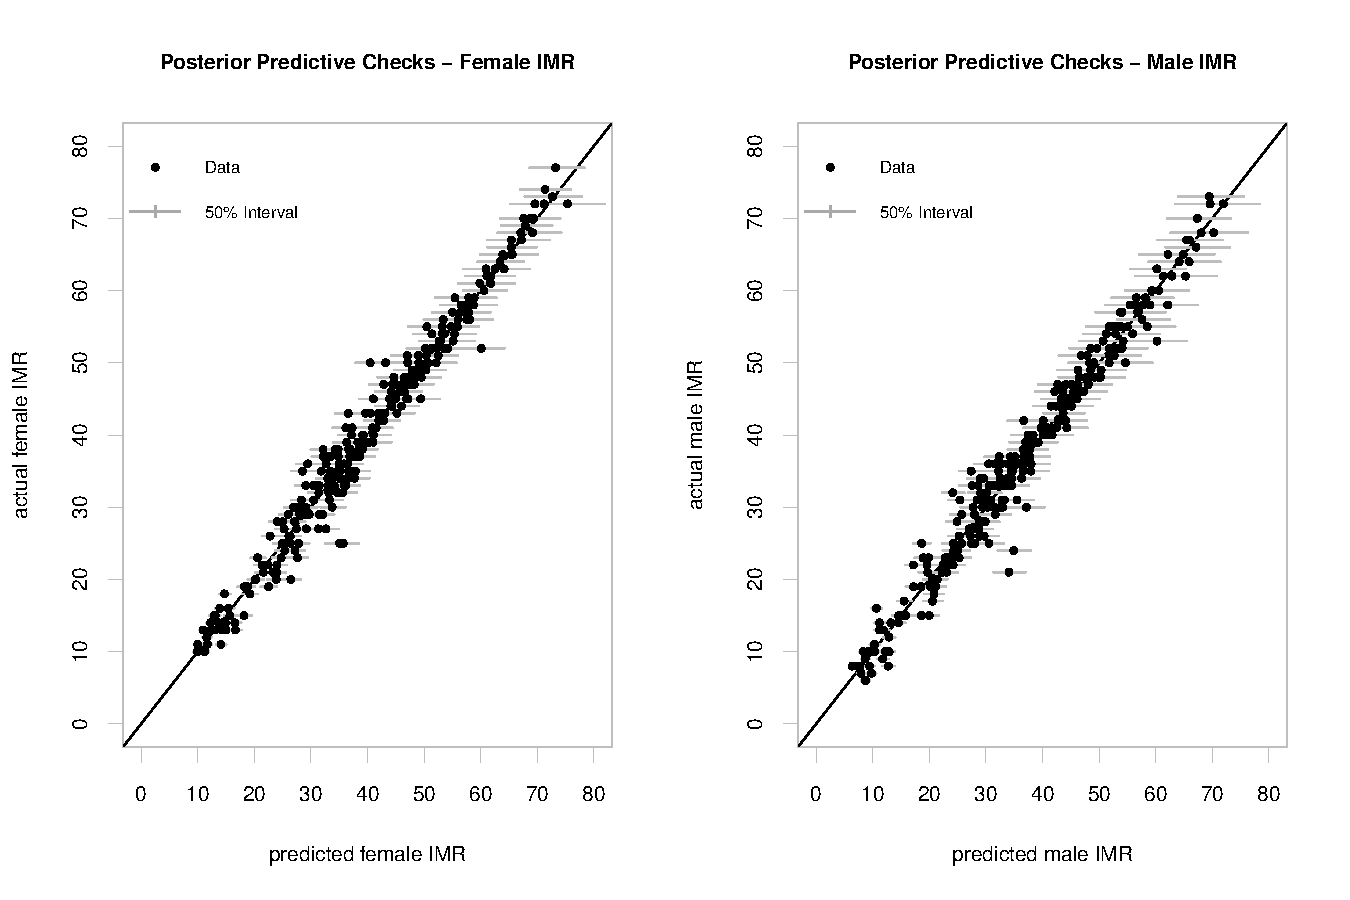
\includegraphics[height = 9cm, width = 15cm]{ppc_1.pdf}
   \end{center}
   \caption{\emph{The horizontal axis shows the predicted IMR and the vertical axis shows the actual IMR for females and males in Fig. 5 (a) and (b) respectively. The black dots show the estimate and the gray lines show the 50\% interval around the estimate.}}
\end{figure}

Figure 5 shows the posterior predictive checking for the dataset as a whole, but for females and males separately as the model was run. The black dots are the estimates and the gray lines around the dots show the 50\% posterior interval around the prediction. The points mostly cluster along the diagonal line which represents the 45$^{\circ}$ line. This shows that the in-sample prediction is pretty good and the model is able predict the IMR values for females and males quite accurately. 

\subsection{Posterior predictive checking for female IMR in the 30 regions from 2006 to 2014}
\begin{figure}[H]
   \begin{center}
   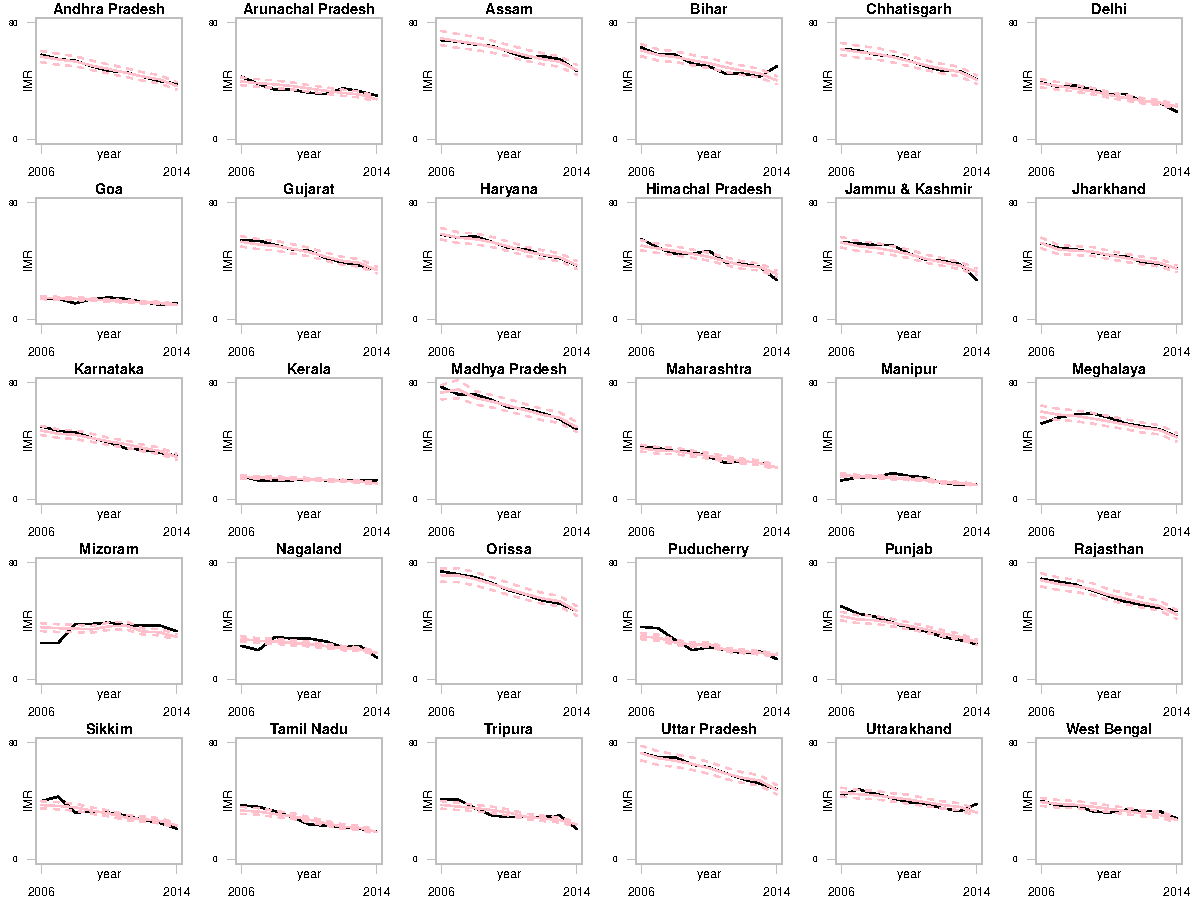
\includegraphics[height = 11cm, width = 15cm]{fem_ppc.pdf}
   \end{center}
   \caption{\emph{The horizontal axis represents years from 2006 to 2014. The vertical axis measures the IMR. The black line shows the true trend in IMR. The solid pink line shows the estimated trend and the dotted pink lines on either side show the 50\% posterior interval.}}
\end{figure}

\subsection{Posterior predictive checking for Male IMR in the 30 regions from 2006 to 2014}
\begin{figure}[H]
   \begin{center}
   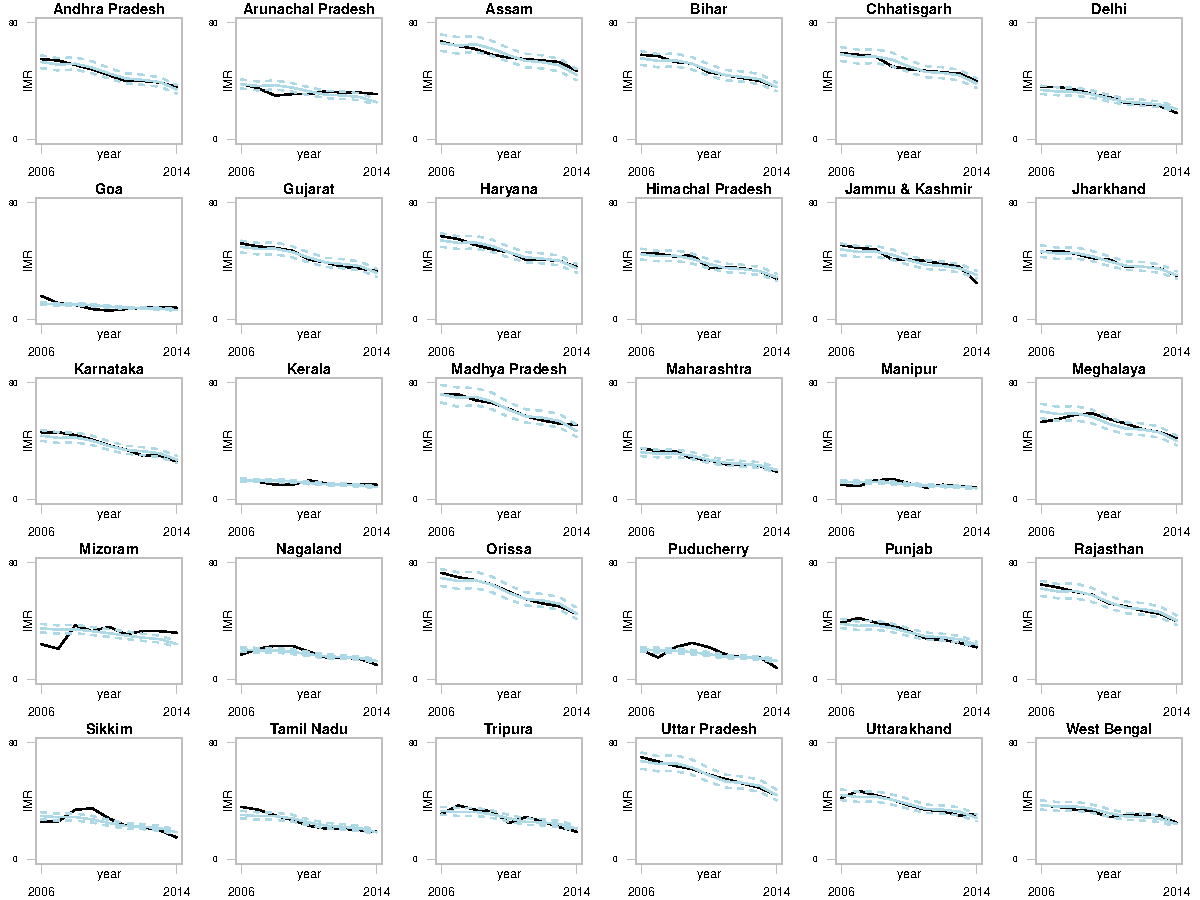
\includegraphics[height = 11cm, width = 15cm]{mal_ppc.pdf}
   \end{center}
   \caption{\emph{The horizontal axis represents years from 2006 to 2014. The vertical axis measures the IMR. The black line shows the true trend in IMR. The solid blue line shows the estimated trend and the dotted blue lines on either side show the 50\% posterior interval.}}
\end{figure}

Figure 6 and 7 are gender wise posterior predictive checks. We observe that the pink lines in Figure 6 and the blue lines in Figure 7 capture the true trend in female and male infant mortalities (respectively). Thus the model performs well in ``learning" the data generating process. Given this information, we are able to examine the parameters more meaningfully and usefully.

\subsection{State level intercepts ($\alpha_s$) for females and males}
\begin{figure}[H]
   \begin{center}
   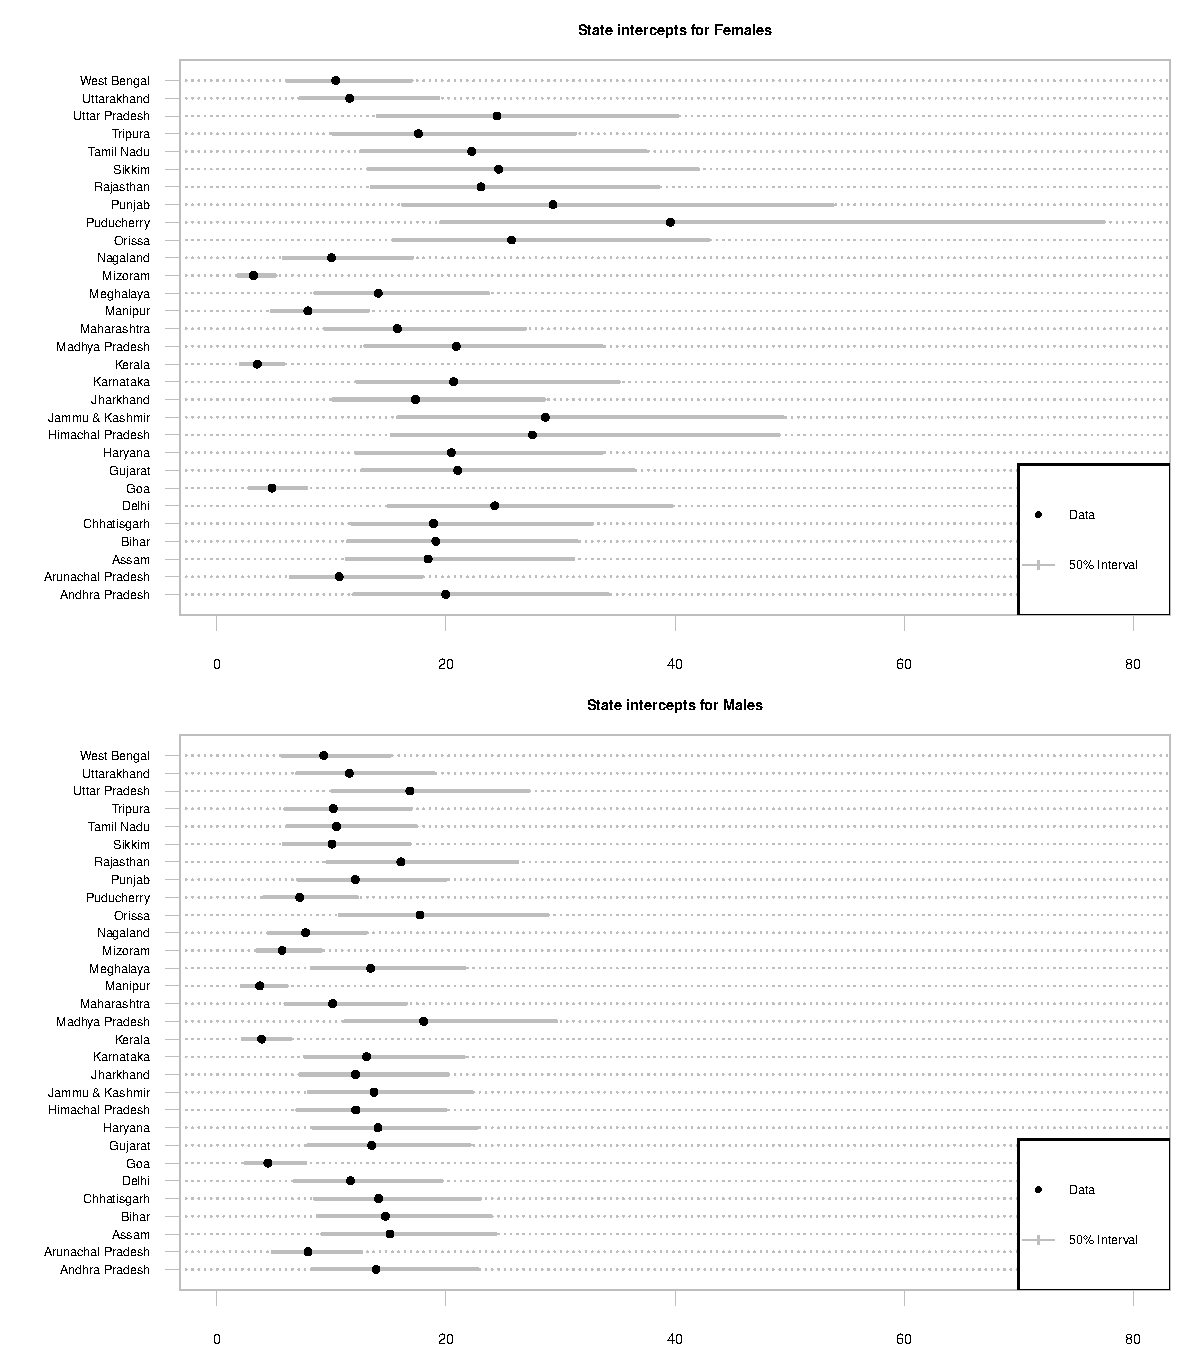
\includegraphics[height = 17cm, width = 15cm]{state_int.pdf}
   \end{center}
   \caption{\emph{The horizontal axes measure IMR. The vertical axes show each of the 30 regions considered. The black dots show the state level estimate of the intercept $\alpha_s$. The gray lines around the black dot show the 50\% posterior interval.}}
\end{figure}
Figure 8 show the state level intercepts $\alpha_s$ for the 30 regions considered for females and males. We notice that estimates of female IMR (in the absence of health expenditure) are higher than male IMR for almost all states. Also we find that states that do well in terms of human development like Kerala and Goa have lower IMR values with shorter intervals and states which tend to perform poorly like Orissa have much wider intervals around their estimate.

\subsection{Marginal posterior distribution of the elasticity parameter ($\beta_s$) for females and males}
\begin{figure}[H]
   \begin{center}
   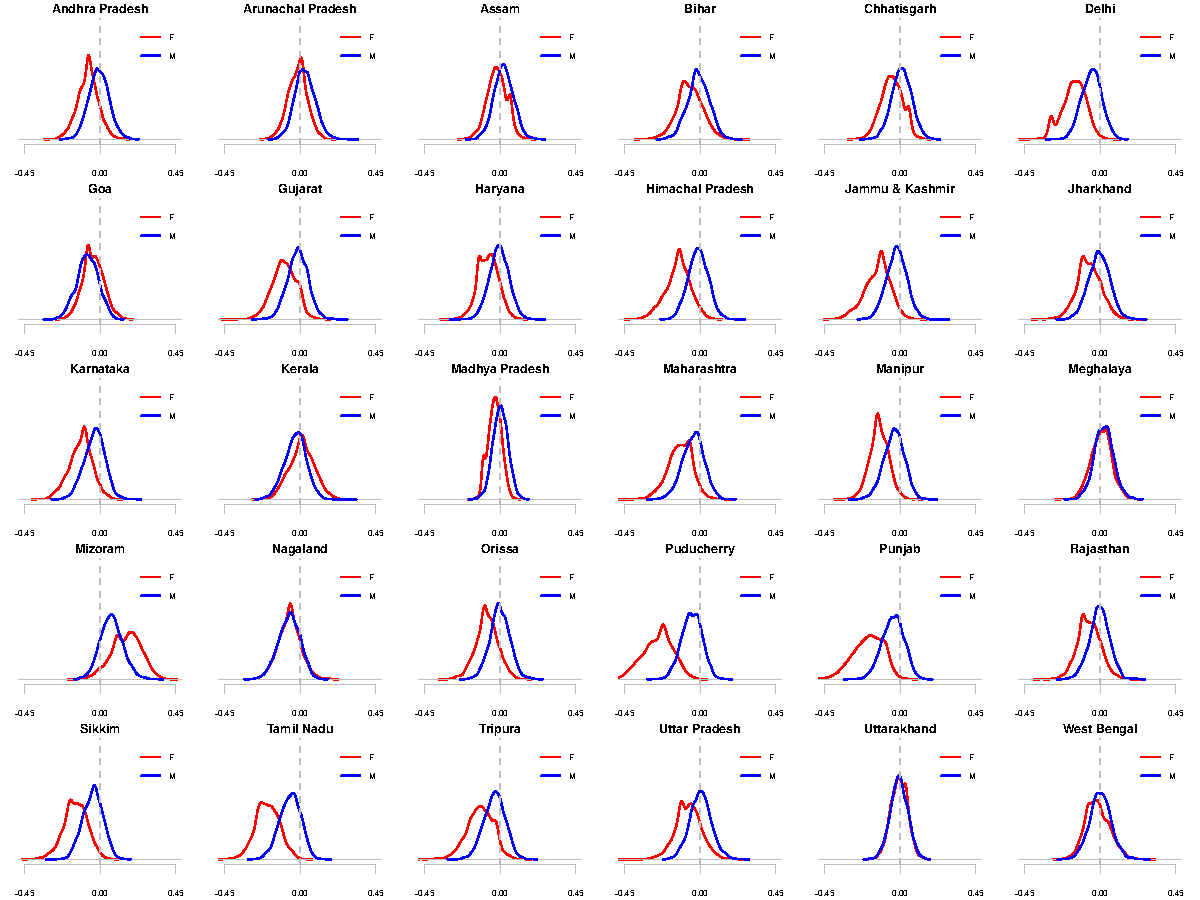
\includegraphics[height = 11cm, width = 15cm]{mar_post.pdf}
   \end{center}
   \caption{\emph{The horizontal axes represent }}
\end{figure}

The marginal posterior of the elasticity in IMR relative to changes in per-capita health expenditure are shown in Figure 9. The red line shows the marginal posterior distribution of $\beta_s$ for females and the blue line shows the marginal posterior distribution of $\beta_s$ for males. We observe that there are distinct patterns for males and females and the behavior of the distribution varies across regions as well. For almost all the regions the elasticity parameter appears to be negative and close to 0. This means that increasing per-capita health expenditure brings down IMR.\\
 This is an important contribution to the methodology in the literature as we have managed to isolate the effect of changing per-capita health expenditure for the 30 regions considered in our study.




%%%%%%%%%%
%    Conclusion  %
%%%%%%%%%%
\section{Conclusion}
In this paper we have studied the Infant Mortality Rate (IMR) in India across 30 states/ Union Territories trying to capture the relationship between state-wise per-capita health expenditure and IMR. We consider data from 2004-2005 to 2013-2014. The data was obtained from publicly available sources. The IMR data comes from the Census Board of India's Sample Registration System (SRS). The data on health expenditure comes from the Reserve Bank of India's State Budget publications and ultimately we calculate per-capita health expenditure for each state and this is our predictor. \\

The contribution this paper makes to the literature on infant mortality, health expenditure and mainly the analysis of panel data is the adoption of a Bayesian framework. The hierarchies in the data structure and the substantial variation in IMR across states and time make a Bayesian multilevel regression model ideal. While previous literature has addressed the `panel' nature of the data, this is the first exhaustive Bayesian analysis. We also go deeper into the nature of IMR by separating it out into male and female IMR in order to examine whether there is a difference in the pattern of deaths between genders.\\

We find that the elasticity of IMR with respect to changes in per-capita health expenditure is indeed negative. This elasticity ($\beta_s$) is different for different states and is also different for female and male infants. For females, $\beta_s \sim \mathcal{N} (-0.08, 0.10)$ and for males $\beta_s \sim \mathcal{N} (-0.02, 0.05)$. However this is a very broad picture and we find (Figure 9) that these trends tend to vary across states. It appears that by using per-capita health expenditure and state level intercepts, we have largely dispersed the state-level variation in health expenditure and thus the real variation in IMR might be due to only state and time variation.\\

The state intercepts $\alpha_s$ turn out to be very different (Figure 8) for all states. We find that the model picks up automatically that female infant deaths are on an absolute level, much higher than male infant deaths. This means that, this is a consistent trend and continues to persist and therefore has to addressed by policy immediately. \\

A critique we can offer of our model is that time periods are not exchangeable units (for example, 2005 and 2014 are not invertible for the purpose of analysis because one happened before the other). This means that alternate methods can be considered for the estimation of such time - level parameters, particularly when time level effects are the quantity of interest. These methods include Bayesian VAR and other Bayesian time series methods. But in our case given the trend in the time period considered was not vastly different and followed a steady declining trend we were able to make this assumption. Another possible advancement of our study is to see how well the model predicts out of sample IMR based on estimates of per-capita health expenditure in order to make sure the model has not been overfit and will in fact generalize to new data. In further extensions we should also consider the rural and urban bifurcation of the IMR in order to see how health expenditure impacts these areas, given the state they are in. This would be a valuable addition to policy information as well.\\


\begin{thebibliography}{9}
\bibitem{Human Development in Poor Countries: On the role of Private Income and Public Services} 
Anand, S. and Ravallion, M (1993).
\textit{``Human Development in Poor Countries: On the role of Private Income and Public Services"}. 
Journal of Economic Perspectives, Volume 7, pp. 133-150.

\bibitem{Spending to Save? State Health Expenditure and Infant Mortality in India}
Bhalotra, S (2007). 
\textit{``Spending to Save? State Health Expenditure and Infant Mortality in India"}
Institute for the Study of Labor : Discussion Paper number - 2914.

\bibitem{Little Girls and Death in India}
Bardhan, P (1982). 
\textit{``Little Girls and Death in India".}
Economic and Political Weekly, Vol. 17, No. 36 (Sep. 4, 1982), pp. 1448-1450

\bibitem{The Effect of Public Health Expenditure on Infant Mortality: Evidence from a Panel of Indian States, 1983?1984 to 2011?2012}
Barenberg, A., Basu, D., Soylu, C. (2016). 
\textit{``The Effect of Public Health Expenditure on Infant Mortality: Evidence from a Panel of Indian States, 1983?1984 to 2011?2012".}
The Journal of Development Studies, DOI: 10.1080/00220388.2016.1241384.

\bibitem{Decomposing Social Indicators Using Distributional Data.}
Bidani, B. and Ravallion, M (1995).
\textit{``Decomposing Social Indicators Using Distributional Data"}
Policy Research Development, The World Bank.

\bibitem{The Differential Effect of
Mothers' Education on Mortality of Boys and Girls in India}
Bourne, K and Walker, G (1991).
\textit{``The Differential Effect of
Mothers' Education on Mortality of Boys and Girls in India,"}
Population Studies, 45:2, 203-219, DOI: 10.1080/0032472031000145396

\bibitem{Country Comparison, Infant Mortality Rate}
Central Intelligence Agency (2014).
\textit{``Country Comparison, Infant Mortality Rate"}

\texttt{https://www.cia.gov/library/publications/the-world-factbook/
rankorder/2091rank.html}

\bibitem{Effects of State-level Public Spending on Health on the mortality Probability in India}
Farahani M, Subramanian S.V, Canning D (2010).
\textit{``Effects of State-level Public Spending on Health on the mortality Probability in India"}
National Institute of Health : Public Access Manuscript .

\bibitem{Hierarchical Models for Causal Effects}
Feller, A and Gelman, A (2015) \textit{``Hierarchical Models for Causal Effects".}
Emerging Trends in the Social and Behavioral Sciences. Edited by Robert Scott and Stephen Kosslyn. ISBN 978-1-118-90077-2.

\bibitem{The impact of public spending on health, Does money matter?}
Filmer and Pritchett (1999),
\textit{``The impact of public spending on health, Does money matter?}
Elsevier, Volume 49, Issue 10,pp 1309 - 1323.

\bibitem{Bayesian Data Analysis}
Gelman A, Carlin J.B, Stern H.S, Rubin D.B (2013).
\textit{``Bayesian Data Analysis"}
ISBN 0-412-03991-5, Chapman and Hall, New York

\bibitem{Multilevel (Hierarchical) Modeling: What It Can and Cannot Do}
Gelman A (2006).
\textit{``Multilevel (Hierarchical) Modeling: What It Can and Cannot Do"}
American Statistical Association and the American Society for Quality TECHNOMETRICS, AUGUST 2006, VOL. 48, NO. 3 DOI 10.1198/004017005000000661.

\bibitem{Prior distributions for variance parameters in hierarchical models(Comment on Article by Browne and Draper)}
Gelman A (2006).
\textit{``Prior distributions for variance parameters in hierarchical models(Comment on Article by Browne and Draper)"}
2006, International Society for Bayesian Analysis, Number 3, pp. 515 - 534.

\bibitem{Public health spending and infant and child mortality in India, a state-year panel analysis}
Kumar K, Singh A, Subramanian S.V (2013).
\textit{``Public health spending and infant and child mortality in India, a state-year panel analysis"}
Munich Personal RePec Archive.

\bibitem{Nationwide children's explaining the country's Infant Mortality Rate}
McLead R (2012).
\textit{Nationwide children's explaining the country's Infant Mortality Rate}
\texttt{http://www.childrensonquality.com/explaining-the-countrys-infant-mortality-rate-part-1/}

\bibitem{Sample Registration System Bulletins}
Ministry of Home Affairs (2014),
\textit{``Sample Registration System Bulletins",}

\bibitem{Reserve Bank of India, State Finances: A Study of Budgets}
Reserve Bank of India
\textit{``State Finances: A Study of Budgets"}
\texttt{https://rbi.org.in/Scripts/AnnualPublications.aspx?head=State\%20Finances\\
\%20:\%20A\%20Study\%20of\%20Budgets}

\bibitem{The Endangered Sex: Neglect of Female Children in Rural North India}
Miller, B (1981).
\textit{``The Endangered Sex: Neglect of Female Children in Rural North India"}
ISBN-13: 9780801413711, Cornell University Press, Ithaca, New York.

\bibitem{Public and Private Roles in Health. Health, Nutrition and Population, Discussion Paper}
Musgrove (1996).
\textit{``Public and Private Roles in Health. Health, Nutrition and Population, Discussion Paper"}
ISBN 1-932126-23-6


\bibitem{The Relationship between Infant Mortality Rate and Health Expenditure in India: A Bayesian Approach}
Rajagopal, A (2016), \textit{``The Relationship between Infant Mortality Rate and Health Expenditure in India: A Bayesian Approach".}
Social Science Research Network. Available at SSRN \texttt{https://ssrn.com/abstract=2788791}

\bibitem{Mortality decline in the low income world, Causes and Consequence}
Schultz, T (1993).
\textit{``Mortality decline in the low income world: Causes and Consequence"}
American Economics Association Annual Meetings, California .

\bibitem{Stan}
Stan Development Team. 2016. 
\textit{RStan: the R interface to Stan}, Version 2.10.1.   
\texttt{http://mc-stan.org}

\bibitem{WHO}
World Health Organization (2013).
\textit{``Global Health Observatory"}



\end{thebibliography}




\end{document}

























